% =================
% Sector Shangra Omega
% =================

\section{Sector Shangra Omega}

\begin{center}
  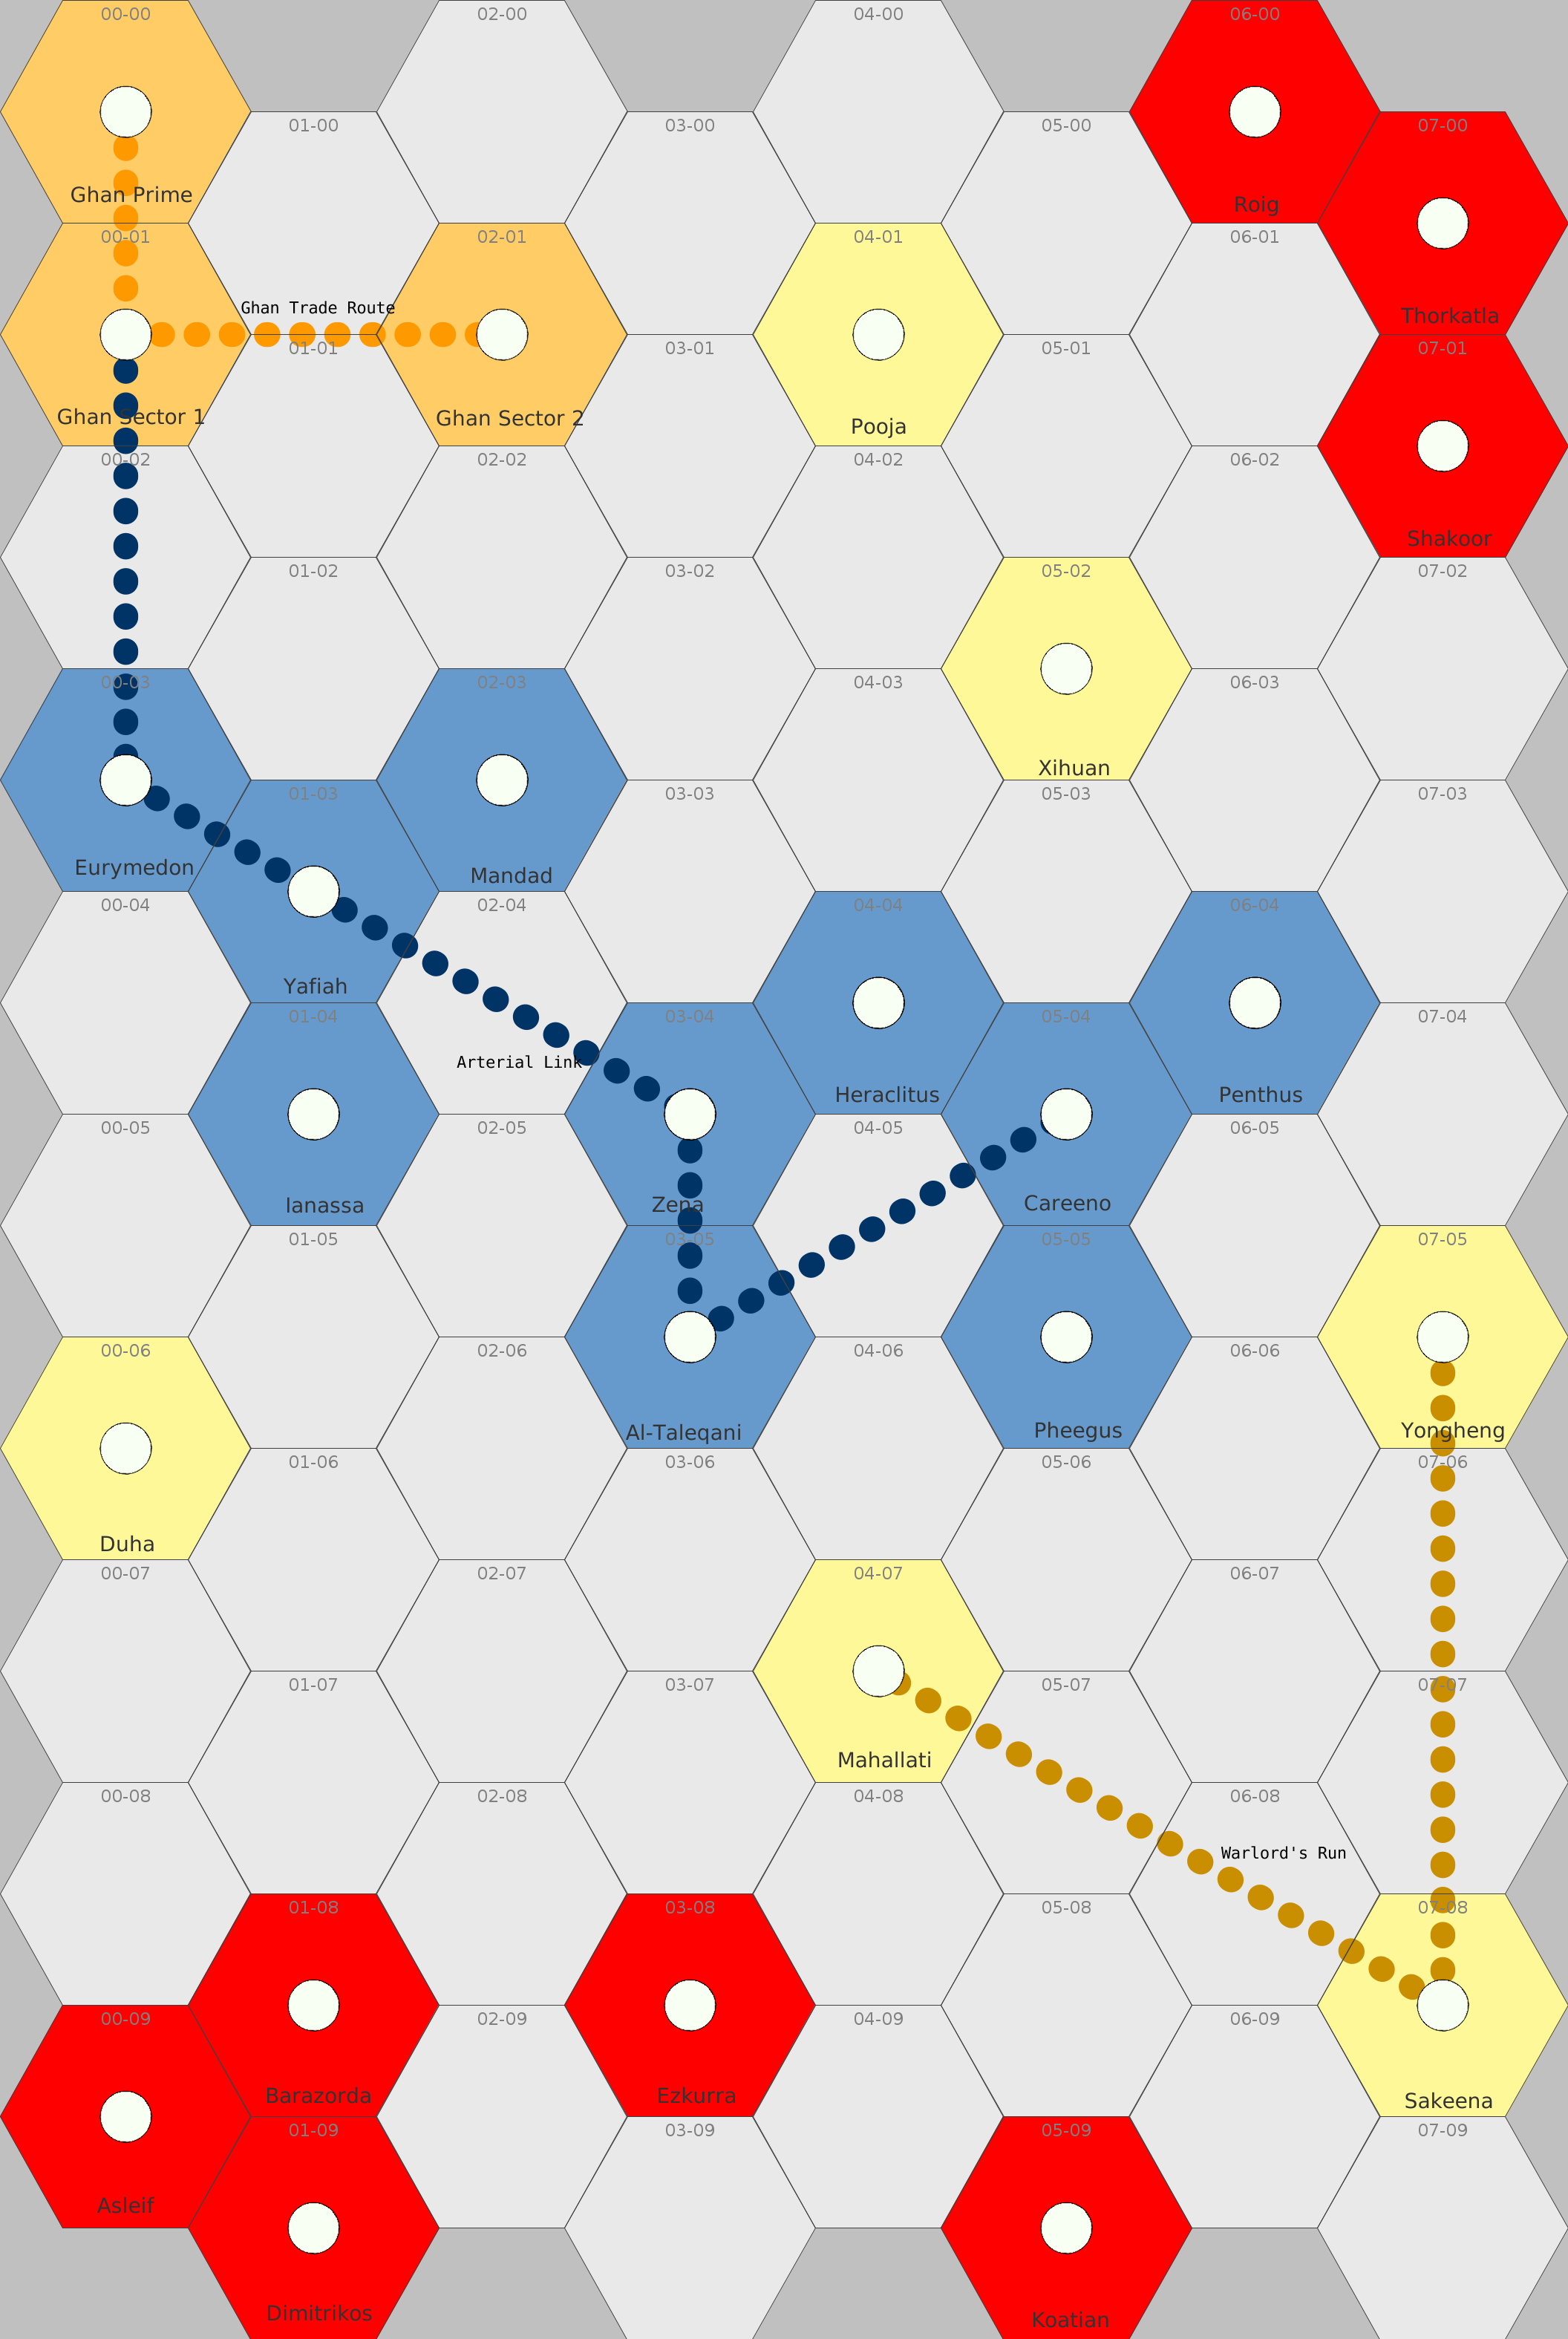
\includegraphics[height=220mm]{sectormap}
\end{center}

\newpage

\begin{multicols}{2}

  \subsection{Star Systems}

  Sector Shangra Omega consists of 10 \textit{Core} systems (blue), 6 \textit{Independent} systems (yellow), 3 \textit{Ghan} systems (orange) and possibly up to 8 \textit{Lost} systems (red). The sectors that surround Shangra Omega are largely unexplored, and ancient star charts are severely out of date. The sector map used by navigators today are the result of intrepid explorers braving the Black and re-charting the stars.

  Core systems are those that make up the \textbf{United Systems}, a loose federation of star systems that share a common legal framework and similar military structures. Planets and Star Systems are allowed to govern themselves, but are subject to Universal Decrees voted upon by the United Systems Council. Each star system sends 10 Delegates to the Council (regardless of the number of planets, colonies, space stations, or other habitation in that system), and Delegates do not necessarily need to be democratically appointed.

  Independent systems are those that choose to remain seperate from the United Systems. Some chose not to join because they feel that the strict 10 Delegates per system would unfairly discriminate their large populations. Others because the Decrees do not align with their local laws and customs. And some wish to remain black market havens. Whatever the reason, Independent systems are considered the "Wild West" of the Black.

  Ghan systems are, quite simply, the home systems for the Ghantak. Ghan Prime has the homeworld of Ghan, and the Ghantak were able to colonise (at least) two other star systems before the Surge. These systems have all managed to survive the Surge and re-establish contact with each other, but choose to remain seperate from the United Systems. They are led by an Empress who resides in Ghan Prime, but each planet is governed by a Hive Queen that has the freedom to do as she pleases.

  Lost systems are those that are speculated to still exist, but no formal communication or expedition exist to explore them fully. Travel to the Lost systems are fraught with danger, as many do not return.

  \columnbreak

  \begin{standardtable}{\linewidth}{bsb}
    \textbf{Name} & \textbf{Sector} & \textbf{Type}\\
    Al-Taleqani & 03-05 & Core\\
    Asleif & 00-09 & Lost\\
    Barazorda & 01-08 & Lost\\
    Careeno & 05-04 & Core\\
    Dimitrikos & 01-09 & Lost\\
    Duha & 00-06 & Independent\\
    Eurymedon & 00-03 & Core\\
    Ezkurra & 03-00 & Lost\\
    Ghan Prime & 00-00 & Ghan\\
    Ghan Sector 1 & 00-01 & Ghan\\
    Ghan Sector 2 & 02-01 & Ghan\\
    Heraclitus & 04-04 & Core\\
    Ianassa & 01-04 & Core\\
    Koatian & 05-09 & Lost\\
    Mahallati & 04-07 & Independent\\
    Mandad & 02-03 & Core\\
    Penthus & 06-04 & Core\\
    Pheegus & 05-05 & Core\\
    Pooja & 04-01 & Independent\\
    Roig & 06-00 & Lost\\
    Sakeena & 07-08 & Independent\\
    Shakoor & 07-01 & Lost\\
    Thorkatia & 07-00 & Lost\\
    Xihuan & 05-02 & Independent\\
    Yafiah & 01-03 & Core\\
    Yongheng & 07-05 & Independent\\
    Zena & 03-04 & Core\\
  \end{standardtable}

  \subsection{Tech-Levels}

  Tech-Levels are a standard way to catergorise the differing manufacturing capabilities of a planet. Some worlds are purposely kept at low tech-levels as they provide primary trade resources for high tech-level worlds (such as agriculture). 

  \begin{standardtable}{\linewidth}{ssb}
    \textbf{Level} & \textbf{Description} & \textbf{Example}\\
    0 & Stone & Stone, human power\\
    1 & Ancient & Metals, domestic animals, steam engine\\
    2 & Industrial & Fossil fuels, factories, simple machines\\
    3 & Mechanized & Computers, satellites, 20th century era tech\\
    4 & Interstellar & IDD, energy weapons, cyberware \\
    5 & Advanced & Specialized knowledge in a technological field\\
    6 & Pre-Surge & Psionic tech, TDD, exotic tech\\
  \end{standardtable}

  \subsection{ATB classification}

  The \textbf{Atmospheric - Temperature - Biosphere} (ATB) rating is the standard classification system for worlds, planets and other naturally occuring stellar bodies. An ATB gives a general overview about the suitability for habitation, or at the very least an idea of what risks there are in colonising the world. The classification uses 3 letters, one for each of the categories of Atmosphere, Temperature and Biosphere.

  \subsubsection{Atmosphere}

  \begin{standardtable}{\linewidth}{sb}
    \textbf{Rating} & \textbf{Description} \\
    A (Airless) & Has no to little atmosphere to speak of\\
    B (Breatheable) & A mix of gases that is within the breatheable range for organic beings. Since each planet has different mixtures, foriegners are always aware of the "new world stink"\\
    C (Corrosive) & Dangerously hostile, even with conventional suits and other protective gear. The atmosphere is extremely toxic, and actively corrodes non-native materials\\
    G (Inert Gas) & Atmosphere consists of gases that are not breatheable by organic beings. The atmosphere is otherwise not hostile or poisonous, but requires a constant source of oxygen\\
    T (Thick) & Can be breathed with the aid of a filtration mask. Usually toxic if an organic decides to breathe the air straight over long periods of time\\
    X (Toxic) & These worlds are much more aggressively hostile than corrosive worlds. These worlds have toxic molecules that are able to bypass suit seals during the corrosion process, meaning that they must be purified at regular intervals, reducing the oxygen supply substantially\\
  \end{standardtable}

  \subsubsection{Temperature}

  \begin{standardtable}{\linewidth}{sb}
    \textbf{Rating} & \textbf{Description} \\
    F (Frozen) & Average temperature that is close to absolute zero. Some are so cold that the gases have solidified\\
    C (Cold) & These worlds are uncomfortably cold, but are survivable with suitable heavy clothing\\
    T (Temperate) & These worlds have temperature ranges that are similar to Earth\\
    W (Warm) & These worlds are uncomfortably warm, but are survivable. They are either desert worlds, or have thick, humid jungles\\
    B (Burning) & Average temperatures that is close to boiling. Some are so hot that metals exist in molten form \\
    V (Varied) & These worlds have a wide range of temperatures, either due to unique geological features or varying orbits around their star\\
  \end{standardtable}

  \subsubsection{Biosphere}

  \begin{standardtable}{\linewidth}{sb}
    \textbf{Rating} & \textbf{Description} \\
    R (Remnants) & The wreckage and ruins of a dead ecology\\
    M (Microbial) & Non-sentient micro-organisms that can exist in almost all types of environments (such as slimes, bacteria, fungus). They may or may not be dangerous \\
    Z (None) & For some reason or other, life did not evolve on this world\\
    C (Compatible) & Substantial portion of native life is biologically compatible with human nutritional needs\\
    I (Incompatible) & None of the native life is biologically compatible with human nutritional needs. Microbial life could potentially be highly allergenic to humans\\
    H (Hybrid) & The native flora and fauna have been intermixed with imported species from Earth. They may or may not be compatible, but are not otherwise hostile\\
    E (Engineered) & Are either paradise planets that have been carefully sculpted, or living forges that produce foodstuffs and minerals for trade\\
  \end{standardtable}

  % PEM Rating
  \subsection{PEM classification}

The \textbf{Politics - Economics - Migration} (PEM) rating is the standard classification system for political entities. An ATB gives a general overview about the political leanings of the organization without resorting to simplified, one-word labels. The classification uses 3 letters, one for each of the categories of Politics, Economics and Migration.

\subsubsection{Politics}

\begin{standardtable}{\linewidth}{sb}
  \textbf{Rating} & \textbf{Description} \\
  O (Outcast) & Targets the outcasts who have been marginalised by society\\
  W (Working) & Targets the working class (both agricultural and industrial)\\
  M (Middle) & Targets the middle class\\
  E (Elite) & Targets the rich and successful, and those aspiring to join it's ranks\\
  T (Traditional) & Targets those who prefer to do things the traditional way (whether culturally, religiously or socially)\\
  P (Progressive) & Targets those who prefer to improve the way things are, regardless of class\\
\end{standardtable}

\subsubsection{Economic}

\begin{standardtable}{\linewidth}{sb}
  \textbf{Rating} & \textbf{Description} \\
  F (Free Market) & Minimal or no government intervention in the market\\
  I (State industry) & The government should own or support important industries\\
  P (Protectionist) & The government should tax imports that threaten to displace local products\\
  S (Socialist) & The market should be harnessed to ensure a state-determined minimal standard of living for all\\
  C (Communist) & The state should control the economy, disbursing its products according to need and determined efficiency\\
  A (Autarky) & The government should ensure that the world can provide all of its own goods and services and forbid the import of foreign goods\\
\end{standardtable}

\subsubsection{Migration}

\begin{standardtable}{\linewidth}{sb}
  \textbf{Rating} & \textbf{Description} \\
  X (Xenophobic) & Immigration is to be restricted to protect native jobs and culture\\
  P (Xenophilia) & More immigrants the better\\
  H (Hybrid) & Some immigrants are to be encouraged, others are forbidden. This list is determined by the government\\
\end{standardtable}

  % Military
  \subsection{Military Ranks}

There will always be a need for a standing military service, and in the Pre-Surge days the powers that be decided on a single rank system for all servicemen (whether army or navy). This standard has been carried on after the Surge, and even warring factions on Independant worlds are known to use the system.

\subsubsection{Enlisted}

Enlisted men provide the manpower for the military services. They serve as the marines, infantry, pilots, engineers, and any other role that is required of them. They can advanced through the ranks in either leadership roles or as specialised experts in their field.

\begin{standardtable}{\linewidth}{sb}
  \textbf{Rank} & \textbf{Duties} \\
  Private (PVT) & The lowest rank\\
  Specialist (SPC) & Used to designate an individual with special skills\\
  Corporal (CPL) & Leader of a team (4 servicemen), or Senior specialists or administrative staff\\
  Sergeant (SGT) & Leader of a section (2-3 teams, 8-15 servicemen), or Senior staff for command-level officers\\
  Master Sergeant (MSG) & Highest rank for non-commissioned officers. Senior staff or supervisors of the enlisted men\\
\end{standardtable}

\subsubsection{Officers}

Officers provide leadership for the men under their command. They command large numbers of men or military spacecraft, and only rise up the ranks through exemplary service.

\begin{standardtable}{\linewidth}{sb}
  \textbf{Rank} & \textbf{Duties} \\
  Ensign (ENS) & Entry-level rank for officers. Generally put in charge of a secion with the aide of a Sergeant\\
  Lietenant (LT) & Leader of a platoon (2-3 sections, 16-45 servicemen), or subordinate for command-level officers\\
  Major (MAJ) & Leader of a company (3-4 platoons, 50-180 servicemen), or commands a small spacecraft\\
  Commander (CDR) & Leader of a battalion (3-4 companies, 200-700), or commands a medium spacecraft\\
  Captain (CPT) & Leader of a brigade (3-4 battalions, 1000-3000), or commands a large spacecraft\\
  Colonel (COL) & Leader of a division (4-5 brigades, 4000-15000), or commands a flotilla (2+ spacecraft)\\
  Vice Admiral (VADM) & Leader of a corps (2-3 divisions, 15000-45000), or commands a group (2+ flotilla). Some infantry forces prefer the older "Lietenant General"\\
  Admiral (ADM) & Leader of an army (2-3 corps, 80000+), or commands a fleet (2+ groups). Some infantry forces prefer the older "General". Seniority is designated by stars, with the highest achievable rank is a 6-star Admiral/General\\
\end{standardtable}

\end{multicols}

\newpage

% Worlds
% =================
% Worlds
% =================
\subsection{Worlds}

  \subsubsection{Core Worlds}

  \begin{powertable}{ p{.10\textwidth} p{.10\textwidth} p{.05\textwidth} p{.05\textwidth} p{.20\textwidth} p{.35\textwidth} }
    \textbf{Name} & \textbf{A-T-B} & \textbf{Pop.} & \textbf{TL} & \textbf{Sector} & \textbf{Tags}\\
    Aerope	    & T-C-H &	10M+  & 3	& Eurymedon (00-03)   & Bigotry, Fear of Psionics\\
    Al-sahhah   & B-V-C & 1B+   & 4 & Al-Taleqani (03-05) & Specialised Technology, Regional Hegemon\\
    Androcles   & B-T-R & 100K+ & 3 & Ianassa (01-04)     & Freak Geology, Quarantined\\
    Arantza     & T-W-C & 1M+   & 4 & Mandad (02-03)      & Restrictive Laws, Primitive Aliens\\
    Ballesteros & T-T-C & 1M+   & 4 & Pheegus (05-05)     & Rigid Culture, Seagoing cities\\
    Bergthora   & A-T-M & 1M+   & 5 & Penthus (06-04)     & Heavy Industry, Theocracy\\
    Hildegunn   & B-W-C &	100K+	& 4	& Ianassa (01-04)     & Pre-Surge Archive, Intelligence\\
    Khadim	    & T-C-I & 100K+ & 3	& Al-Taleqani (03-05) & Gold Rush, Colonised\\
    Mahats	    & T-T-E &	100K+ &	4 & Careeno (05-04)     & Agriculture, Theocracy\\
    Marider	    & A-T-R & 10M+	& 5	& Zena (03-04)        & Heavy Mining, Major Spaceyard\\
    Mecisteus   & B-T-C & 100M+ & 4 & Yafiah (01-03)      & Banking, Local Specialiaty\\
    Merlo       & B-T-I & 1M+   & 3 & Mandad (02-03)      & Psionic School, Quarantined\\
    Nishtha     &	B-C-C &	100K+	& 4	& Eurymedon (00-03)   & Pre-Surge Ruins, Pilgrimage\\
    Olaria      & G-T-C & 10M+  & 5 & Eurymedon (00-03)   & Pre-Surge Cultists, Xenophiles\\
    Orithyia    & G-T-E &	100K+	& 4	& Pheegus (05-05)     & Altered Humans, Agriculture\\
    Parezi	    & A-W-M & 1M+	  & 4	& Heraclitus (04-04)  & Heavy Mining, Bubble Cities\\
    Polypheme	  & G-V-I & 10M+  &	4 & Careeno (05-04)     &	Trade Hub, Specialised AI\\
    Raghd       & B-T-Z & 1B+   & 5 & Carreno (05-04)     & Flying Cities, Major Spaceyard\\
    Semera      & B-V-I &	100K+	& 4	& Penthus (06-04)     & Outpost, Police State\\
    Thurid      & B-C-C & 100M+ & 4	& Zena (03-04)        & Trade Hub, Heavy Industry\\
  \end{powertable}
 
  \subsubsection{Independent Worlds}

  \begin{powertable}{ p{.10\textwidth} p{.10\textwidth} p{.05\textwidth} p{.05\textwidth} p{.20\textwidth} p{.35\textwidth} }
    \textbf{Name} & \textbf{A-T-B} & \textbf{Pop.} & \textbf{TL} & \textbf{Sector} & \textbf{Tags}\\
    Amir        & B-T-C & 1M+   & 4 & Duha (00-06)      & Oceanic World, Fear of Psionics\\
    Ba'albaki	  & B-C-H &	1M+   &	4	& Xihuan (05-02)    & Psionic School, Psionic Worship\\
    Dirce       & B-V-C & 100K+ & 4 & Pooja (04-01)     & Desert World, Civil War\\
    Garrastazu  & T-T-H & 1M+   & 3 & Duha (00-06)      & Violent Sectarians, Heavy Mining\\
    Georghiou	  & B-T-E & 1M+   &	3 &	Sakeena (07-08)   & Colonised, Agriculture\\
    Oeneus      & G-T-I & 1M+   & 3 & Sakeena (07-08)	  & Colonised, Heavy Industry\\
    Sakeena     & T-T-I & 10B+  & 5 & Sakeena (07-08)   & Major Spaceyard, Police State\\
    Salimah	    & B-T-E & 100K+ &	4	& Mahallati (04-07) & Rigid Culture, Eugenic Cultists\\
    Theano      & B-F-H & 100K+ & 3 & Yongheng (07-05)  & Outpost, Hatred\\
    Thorhalla   & T-V-H & 10M+  & 4 & Xihuan (05-02)    & Tyranny, Bigotry\\
    Vinata      & G-W-C & 1M+   & 4 & Mahallati (04-07) & Civil War, Bubble Cities\\
    Vargos      & T-T-H & 1B+   & 3 & Yongheng (07-05)  & Cold War, Warlords\\
  \end{powertable}

  \subsubsection{Lost Worlds}

  \begin{powertable}{ p{.10\textwidth} p{.10\textwidth} p{.05\textwidth} p{.05\textwidth} p{.20\textwidth} p{.35\textwidth} }
    \textbf{Name} & \textbf{A-T-B} & \textbf{Pop.} & \textbf{TL} & \textbf{Sector} & \textbf{Tags}\\
    Akriti      & A-T-C & ?     & ? & Koatian (05-09)     & Zombies, Out of Contact\\
    Chloe       & B-T-C & 100K+ & 2 & Ezkurra (03-08)     & Minimal Contact, Fear of Tech\\
    Echepolos   & ?-T-M & ?     & ? & Shakoor (07-01)     & Radioactive, Tomb World\\
    Gyda        & B-C-C & 10K+  & 3 & Aslief (00-09)      & Xenophobes, Pre-Surge Archive\\
    Maqsood     & B-C-H & 100K+ & 3 & Dimitrikos (01-09)  & Psionic Worship, Out of Contact\\
    Purva       & B-F-C & 100K+ & 3 & Barazorda (01-08)   & Feral, Pre-Surge Cultists\\
    Pylaimenos  &	A-V-Z & ?     &	? & Thorkatia (07-00)   &	Sealed Menace, Unbreaked AI\\
    Sagari      & B-T-C & 10K+  & 4 & Shakoor (07-01)     & Hostile Space, Badlands World\\
    Xanthippe	  & B-T-H &	1M+   &	4	& Roig (06-00)        & Tyranny, Theocracy\\
  \end{powertable}

  \subsubsection{Ghan Worlds}

  \begin{powertable}{ p{.10\textwidth} p{.10\textwidth} p{.05\textwidth} p{.05\textwidth} p{.20\textwidth} p{.35\textwidth} }
    \textbf{Name} & \textbf{A-T-B} & \textbf{Pop.} & \textbf{TL} & \textbf{Sector} & \textbf{Tags}\\
    Ghalla	& B-W-C &	100K+	& 4	& Ghan Sector 1 (00-01) & Trade Hub, Local Speciality\\
    Ghan    & B-T-C & 10B+  & 5 & Ghan (00-00)          & Banking, Regional Hegemon\\
    Ghatla	& T-W-C &	100K+	& 4	& Ghan (00-00)          & Freak Weather, Agriculture\\
    Gharda  &	B-W-C & 100K+ &	4	& Ghan Sector 2 (02-01) & Oceanic, Major Spaceyard\\
    Ghusha	& A-C-M	& 100K+ &	4	& Ghan Sector 2 (02-01) & Heavy Mining, Freak Geology\\
  \end{powertable}

% Business groups and factions
% =================
% BUSINESS GROUPS AND FACTIONS
% =================
\subsection{Corporations}
  
  \subsubsection{Core Corporations}

  \begin{powertable}{ p{.20\textwidth} p{.35\textwidth} p{.35\textwidth} }
    \textbf{Business} & \textbf{Name} & \textbf{Headquarters}\\
    Agriculture   & Tatum Farming Collective  & Arantza, Mandad (02-03)\\
    Agriculture   & Aqualis Food Conglomerate & Mahats, Careeno (05-04)\\
    Agriculture   & SuriTech Foodstuffs       & Orithyia, Pheegus (05-05)\\
    Astronautics  & Mavridou Cooperative      & Raghd, Careeno (05-04)\\
    Astronautics  & Quebe-Luxfause Systems    & Marider, Zena (03-04)\\
    Biotech       & Interstellar Genetics Inc & Mahats, Careeno (05-04)\\
    Biotech       & Morgath Industries        & Khadim, Al-Taleqani (03-05)\\
    Biotech       & Umbrella Coorporation     & Ballestreros, Pheegus (05-05)\\
    Construction  & Novaplex                  & Mecisteus, Yafiah (01-03)\\
    Construction  & Panstellar Zaibatsu       & Bergthora, Penthus (06-04)\\
    Cybernetics   & Imaharatronics            & Olaria, Eurymedon (00-03)\\
    Cybernetics   & Lacuna, Inc.              & Hildegunn, Ianassa (01-04)\\
    Cybernetics   & Wayne Enterprises         & Thurid, Zena (03-04)\\
    Electronics   & Altin Alliance            &	Polypheme, Careeno (05-04)\\
    Electronics   & Gowix Computers           & Hildegunn, Ianassa (01-04)\\
    Electronics   & MicroData Technologies    & Al-sahhah, Al-Taleqani (03-05)\\
    Entertainment & Al-Rhul Productions       &	Al-sahhah, Al-Taleqani (03-05)\\
    Entertainment & Haen Multistellar         & Olaria, Eurymedon (00-03)\\
    Exploration   & Bellixan Endeavors        & Khadim, Al-Taleqani (03-05)\\
    Exploration   & Degan Explorations        & Nishtha, Eurymedon (00-03)\\
    Finance       & Anistonopoulos Clan       & Mecisteus, Yafiah (01-03)\\
    Finance       & Gringotts                 & Mecisteus, Yafiah (01-03)\\
    Fishing       & Nopoulos Partnership      & Ballesteros, Pheegus (05-05)\\
    Fuel Refinery & Burns Industries          & Raghd, Careeno (05-04)\\
    Fuel Refinery & Parezi Energy             & Parezi, Heraclitus (04-04)\\
    Genetics      & Gentik                    & Bergthora, Penthus (06-04)\\
    Genetics      & Orithyia Genetics         & Orithyia, Pheegus (05-05)\\
    Genetics      & Nazari Cooperative        & Olaria, Eurymedon (00-03)\\
    Manufacturing & Gorallis Metalworking     & Raghd, Careeno (05-04)\\
    Manufacturing & Kroeskin Fabrications     & Thurid, Zena (03-04)\\
    Manufacturing & Merr-Sonn Industrial      & Al-sahhah, Al-Taleqani (03-05)\\
    Mining        & Colonial Mining           & Parezi, Heraclitus (04-04)\\
    Mining        & Nexcore Mining Corp       & Marider, Zena (03-04)\\
    Pharma.       & Saraphis Megacorp         & Mecisteus, Yafiah (01-03)\\
    Pharma.       & Velunza Circle            & Olaria, Eurymedon (00-03)\\
    Programming   & HoloGraphics Interstellar & Mecisteus, Yafiah (01-03)\\
    Programming   & Perzome SoftWEAR          & Olaria, Eurymedon (00-03)\\
    Programming   & Pied Piper                & Hildegunn, Ianassa (01-04)\\
    Robotics      & Advanced Ideas Mechanics  & Marider, Zena (03-04)\\
    Robotics      & Aperture Science, Inc.    & Thurid, Zena (03-04)\\
    Robotics      & Cyberdyne Systems         & Bergthora, Penthus (06-04)\\
    Security      & Asset Group Solutions     & Al-sahhah, Al-Taleqani (03-05)\\
    Security      & Barichello Multistellar   & Semera, Penthus (06-04)\\
    Security      & Santhe Security           & Mecisteus, Yafiah (01-03)\\
    Spacecraft    & Curich Engineering        & Marider, Zena (03-04)\\
    Spacecraft    & Ferris Spacecraft         & Marider, Zena (03-04)\\
    Spacecraft    & Solar Spacecraft          & Raghd, Careeno (05-04)\\
    Spacecraft    & Starlette Industries      & Raghd, Careeno (05-04)\\
    Snacks        & Buy n Large               & Thurid, Zena (03-04)\\
    Snacks        & Los Pollos Hermanos       & Al-sahhah, Al-Taleqani (03-05)\\
    Weapons       & Al-Astra Association      & Al-sahhah, Al-Taleqani (03-05)\\
    Weapons       & Stark Industries          & Thurid, Zena (03-04)\\
  \end{powertable}
  
  \subsubsection{Independant Coorporations}
  
  \begin{powertable}{ p{.25\textwidth} p{.35\textwidth} p{.35\textwidth} }
    \textbf{Business} & \textbf{Name} & \textbf{Headquarters}\\
    Fishing       & Faraj Fishing             & Amir, Duha (00-06)\\
    Illicit Drugs & Zea Outfit	              & Vinata, Mahallati (04-07)\\
    Illicit Drugs & Spiker Group              & Dirce, Pooja (04-01)\\
    Piracy        & Magnus Syndicate          & Sagari, Shakoor (07-01)\\
    Spacecraft    & Ghan Spacecraft           & Gharda, Ghan Sector 2 (02-01)\\
    Spacecraft    & Sakeena Shipyards         & Sakeena, Sakeena (07-08)\\
    Weapons       & Cafu Pact                 & Dirce, Pooja (04-01)\\
    Weapons       & Jayhoon Faction           & Vinata, Mahallati (04-07)\\
    Weapons       & Striker Ring              & Sagari, Shakoor (07-01)\\
    Weapons       & West Wind Outfit          & Vargos, Yongheng (07-05)\\
    Xenotech      & Ghan Systems              & Ghalla, Ghan Sector 1 (00-01)\\
  \end{powertable}

% Political groups and factions
% =================
% POLITICAL GROUPS AND FACTIONS
% =================
\subsection{Politics}
  
\subsubsection{United Planet Factions}

\begin{redpowertable}{ p{.20\textwidth} p{.05\textwidth} p{.25\textwidth} p{.4\textwidth} }
  \textbf{Name} & \textbf{Seats} & \textbf{Homeworld} & \textbf{Issues}\\
  Buffalo Party     & 5   & Arantza, Mandad (02-03)         & Culture, Traditionalists, Free Market \\
  Cerulean Guild    & 2   & Mecisteus, Yafiah (01-03)       & Progressives, Government reform, Industrial reform, Free Market\\
  Cobalt Consensus  & 7   & Raghd, Careeno (05-04)          & Industrialists, Welfare, Xenophiles \\
  Democratic Party	& 13  & Thurid, Zena (03-04)            &	Government reform, Foreign Policy, Xenophiles\\
  Freedom Element	  & 1   & Mecisteus, Yafiah (01-03)       &	Elitists, Foreign Policy, Protectionist, Autarky (Self-sufficiency), Xenophobia\\
  Homeland Alliance	& 3   & Ballesteros, Pheegus (05-05)    & Bigotry, Culture, Traditionalists, Protectionists\\
  Iron Front	      & 11  & Parezi, Heraclitus (04-04)      &	Working Class, Protectionist, Poverty, Welfare\\
  Libertarian       & 5   & Mecisteus, Yafiah (01-03)       & Progressive, Individual Rights, Industrial reform, Free Market, Xenophiles\\
  Liberty Combine	  & 15  & Al-sahhah, Al-Taleqani (03-05)  &	Foreign Policy, Free Market, Individual Rights\\
  Fellowship        & 3   & Hildegunn, Ianassa (01-04)      &	Progressives, Socialists, Foriegn Policy, Individual Rights\\
  Popular Banner    & 5   & Aerope, Eurymedon (00-03)       &	Working Class, Bigotry, Immigration, Autarky (self-sufficiency)\\
  Psionic Union	    & 3   & Merlo, Mandad (02-03)           &	Psionics, Communists, Government Reform, Individual Rights\\
  Social Federation & 6   & Raghd, Careeno (05-04) 	        & Culture, Industry\\
  Tyrian Consensus	& 4   &	Bergthora, Penthus (05-04)      & Religion, Tradition\\
  Unified Planets   & 11  & Al-sahhah, Al-Taleqani (03-05)  &	Foriegn Policy, Military\\
  Victory Sodality	& 6   & Semera, Penthus (05-04)         &	Traditionalists, State Industry, Military\\
\end{redpowertable}

\begin{multicols}{2}

\subsubsection{Organised Religions}

\begin{genericsection}{Earth Standard}
Earth Standard is a loose classification for any religious system that can trace it's roots back to Earth. Religious belief is one of the few things people hang on to when trying to survive, and many stubbornly refuse to change. These religious beliefs are usually passed down from close family members or friends. Religions include Buddhism, Christianity, Hinduism, Islam, Jews, and Mormonism.
\end{genericsection}

\begin{genericsection}{Neofundamentalist Ideologists}
\textbf{No universal leadership}\\
Born in the classical philosphical teachings of Earth (especially Stoicism). NFI adherants believe in accepting your lot in life, actively resisting temptation, and using Science to further our understanding of the world
\end{genericsection}

\begin{genericsection}{New Catholics}
\textbf{Ruling Council on Bergthora, Penthus}\\
Cut off from the Vatican (and Earth), the primarily Catholic colony at Bergthora created their own Council of Cardinals to provide leadership for their faithful. The Council gradually took over the governance of the entire system. New Catholics are the largest Christian organisation in the sector, mainly because they accept differing ideas on the nature of God and were able to adopt practices of other Christians
\end{genericsection}

\begin{genericsection}{Quietist Muslims}
\textbf{Communal Democracy}\\
Largely concentrated on Mahats in the Careeno system. After the turbulent 21st Century, the Islamic faith began to reject the old power structures and began to democratically guide their faith in the best interests of the community. The faith largely shuns foriegn policy issues that do not affect their world, and strives to limit their involvement with the affairs of nonbelievers. They prefer to keep to their own kind and avoid positions of wealth and power
\end{genericsection}

\begin{genericsection}{Stellarist Muslims}
\textbf{Communal Democracy}\\
Largely concentrated on Mahats in the Careeno system. A reaction to the Quietist movement, Stellarists believe that the movement has drifted too far from the original teachings. Stellarists desire to reintegrate the Islam faith within the larger interstellar community, and allow their members to actively seek positions of power and wealth
\end{genericsection}

\begin{genericsection}{Syncretism}
\textbf{No universal leadership}\\
After the Surge, many colonies began to focus on survival instead of religious fundamentals. This has resulted in many planets mixing and matching tenets from a wide spectrum of beliefs. This is the most common religion found within the sector
\end{genericsection}

\end{multicols}

